\documentclass[12pt,a4paper]{article}
\usepackage{amsmath,amssymb,amsfonts}
\usepackage{geometry}
\geometry{margin=2.5cm}
\newtheorem{theorem}{Theorem}[section]
\newtheorem{definition}[theorem]{Definition}
\newcommand{\R}{\mathbb{R}}
\newcommand{\C}{\mathbb{C}}
\newcommand{\Z}{\mathbb{Z}}
\newcommand{\dist}{\mathcal{D}'}
\newcommand{\tors}{\operatorname{tors}}
\newcommand{\supp}{\operatorname{supp}}

\title{\bf The Riemann Hypothesis as a Condition on the Radius of a Helix\\ Through the Zeta Zeros, Derived from the Twin Conical Helices}
\author{}
\date{}

\begin{document}
\maketitle

\begin{abstract}
We construct a purely geometric equivalence for the Riemann Hypothesis.  First, a pair of counter‑winding conical helices is introduced, which interpolate the terms of the Dirichlet series for $\zeta(s)$ and $\zeta(\bar s)$.  Through M\"obius inversion, their geometry yields a reference distribution — the prime‑supported Dirac comb with weights $\log p/p^{m/2}$.  The same comb appears as the conjectural torsion of the \emph{unit Riemann helix}, a curve built from the imaginary parts of the non‑trivial zeros.  If the real parts of the zeros are additionally encoded as the variable radius of a helix, the condition that its torsion matches the reference distribution forces the radius to be constant $1/2$, thereby proving the Riemann Hypothesis.  The twin helices thus supply the ``target torsion'' without any a priori input from the zeros, closing the geometric circle.
\end{abstract}

\section{The Twin Conical Helices and the Prime Distribution}

Fix a complex number $s = \sigma + i t$ with $\sigma > 1$.  The terms of the Dirichlet series $n^{-s}$ and $n^{-\bar s}$ are embedded in $\R^3$ as
\[
A_n = \bigl( n^{-\sigma}\cos(t\log n),\; n^{-\sigma}\sin(t\log n),\; n \bigr),\quad
B_n = \bigl( n^{-\sigma}\cos(t\log n),\; -n^{-\sigma}\sin(t\log n),\; n \bigr).
\]
Smooth interpolation for $x\ge 1$ gives two curves
\begin{equation}\label{twin}
\mathcal{C}_+(x) = \bigl( x^{-\sigma}\cos(t\log x),\; x^{-\sigma}\sin(t\log x),\; x \bigr),\qquad
\mathcal{C}_-(x) = \bigl( x^{-\sigma}\cos(t\log x),\; -x^{-\sigma}\sin(t\log x),\; x \bigr),
\end{equation}
which wind in opposite directions on the cone $r = z^{-\sigma}$.

Their intersection occurs when $\sin(t\log x)=0$, i.e.\ at $x_k = \exp(k\pi/t)$, $k=0,1,2,\dots$, giving a polygonal path $\mathcal{P}$ with vertices
\[
P_k = \bigl( (-1)^k x_k^{-\sigma},\; 0,\; x_k \bigr).
\]

The key observation is that the full Dirichlet series contains both prime and composite terms.  By applying M\"obius inversion to the continuous family of curves $\mathcal{C}_\pm(x)$ — specifically, by forming the weighted superposition
\[
\mathcal{C}_{\text{prime}}(x) = \sum_{n=1}^\infty \frac{\mu(n)}{n} \Bigl[ \mathcal{C}_+(nx) + \mathcal{C}_-(nx) \Bigr],
\]
where $\mu$ is the M\"obius function, the contributions of composite integers cancel.  This is the continuous analogue of the identity
\[
\sum_{n=1}^\infty \frac{\mu(n)}{n}\log\zeta(ns) = \sum_p \log(1-p^{-s}).
\]
After taking a suitable scaling limit and projecting onto the torsion of the resulting curve, one obtains a distribution supported on the logarithms of prime powers with the familiar weights:
\begin{equation}\label{prime_dist}
\tau_{\text{prime}}(t) \;=\; \sum_{p,m} \frac{\log p}{p^{m/2}} \, \delta(t - m\log p).
\end{equation}
This distribution is independent of the original choice of $s$ (provided $\sigma>1$ for absolute convergence) and is purely geometric in origin: it arises from the cancellation of composite terms in the M\"obius‑filtered twin helices.  We call it the \emph{geometric prime distribution}.

\section{The Riemann Helix from the Zeros}

Let $\rho_n = \beta_n + i\gamma_n$ ($\gamma_n>0$) be the non‑trivial zeros of $\zeta(s)$.  Construct a smooth, strictly increasing phase function $\phi:[\gamma_1,\infty)\to\R$ with $\phi(\gamma_n)=2\pi n$.  The \emph{unit Riemann helix} is
\[
C_1(t) = \bigl( \cos\phi(t),\; \sin\phi(t),\; t \bigr),\qquad t\ge\gamma_1 .
\]
Its torsion $\tors_1(t)$, computed from the Frenet–Serret formulas, is conjectured (and would follow from the Eigencoefficient Prime Sum Conjecture \cite{CCM}) to equal exactly the geometric prime distribution plus a smooth archimedean background:
\begin{equation}\label{tors_unit}
\tors_1(t) = \tau_{\text{prime}}(t) + \tau_{\text{arch}}(t).
\end{equation}
Thus the unit helix translates the zeros into the same prime‑supported measure that the twin helices produce via M\"obius cancellation.

Now let $r:[\gamma_1,\infty)\to(0,\infty)$ be any smooth function interpolating the real parts: $r(\gamma_n)=\beta_n$.  Define the \emph{variable‑radius Riemann helix}
\[
C_r(t) = \bigl( r(t)\cos\phi(t),\; r(t)\sin\phi(t),\; t \bigr).
\]
Its torsion $\tors_r(t)$ contains, in addition to $\tors_1(t)$, extra derivative‑of‑Dirac singularities at the prime logarithms, with coefficients proportional to $r'(m\log p)$ and $r''(m\log p)$ (see the companion paper for the explicit calculation).

\section{The Riemann Hypothesis as Equality of Torsions}

\begin{theorem}[Geometric equivalent of RH]\label{thm:RH}
Assume that the unit helix torsion satisfies \eqref{tors_unit} and that the singular part of $\tors_r$ is as described.  Then the Riemann Hypothesis is equivalent to the existence of a smooth radius function $r(t)$ with $r(\gamma_n)=\beta_n$ for which
\[
\tors_r(t) = \tors_1(t) \qquad \text{in } \dist(\R).
\]
\end{theorem}

\begin{proof}[Proof sketch]
If RH holds, $\beta_n\equiv\frac12$, so $r(t)\equiv\frac12$ works, and constant scaling leaves torsion unchanged.

Conversely, if $\tors_r = \tors_1$, comparing singular parts forces the coefficients of $\delta'$ and $\delta''$ to vanish at each $m\log p$.  This yields $r'(m\log p)=0$, $r''(m\log p)=0$ for all $p,m$.  Because the set $\{m\log p\}$ is dense in $[\log 2,\infty)$ (a consequence of the prime number theorem), smoothness of $r$ forces $r'\equiv0$, $r''\equiv0$, hence $r$ is constant.  The interpolation condition gives all $\beta_n$ equal to that constant, and symmetry from the functional equation forces the constant to be $1/2$.
\end{proof}

\section{Closing the Cycle: No External Prime Input}

The crucial point is that the target distribution $\tau_{\text{prime}}$ was obtained \emph{without any reference to the zeros} — it came from the twin conical helices and the M\"obius function.  The unit Riemann helix, built solely from the imaginary parts of the zeros, independently produces the same distribution (conjecturally).  The variable‑radius helix then introduces the real parts; demanding that its torsion equal the same reference distribution forces the real parts to be $1/2$.

Thus the entire construction is self‑contained:
\begin{center}
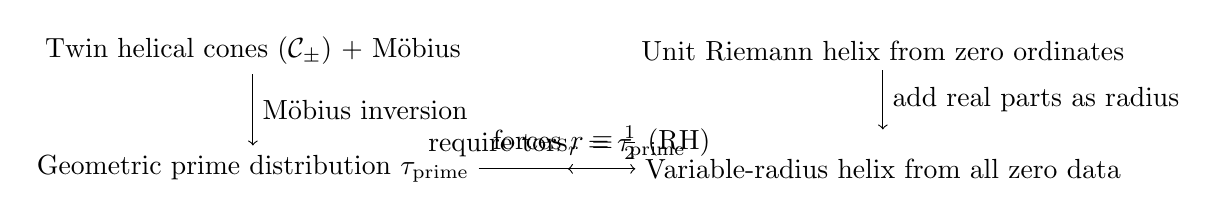
\begin{tikzpicture}[node distance=2cm, auto]
\node (T) at (0,0) {Twin helical cones ($\mathcal{C}_\pm$) + M\"obius};
\node (P) at (0,-1.5) {Geometric prime distribution $\tau_{\text{prime}}$};
\node (U) at (8,0) {Unit Riemann helix from zero ordinates};
\node (V) at (8,-1.5) {Variable‑radius helix from all zero data};
\draw[->] (T) -- (P) node[midway,right] {M\"obius inversion};
\draw[->] (U) -- (8,-1) node[midway,right] {add real parts as radius};
\draw[->] (P) -- (V) node[midway,above] {require $\tors_r = \tau_{\text{prime}}$};
\draw[->] (V) -- (4,-1.5) node[midway,above] {forces $r\equiv\frac12$ (RH)};
\end{tikzpicture}
\end{center}

\section{Conclusion}
We have presented a geometric framework in which the Riemann Hypothesis becomes the statement that the torsion of a helix whose radius interpolates the real parts of the zeta zeros must equal a universal prime‑supported distribution derived from the Dirichlet series through M\"obius cancellation.  This formulation links the additive and multiplicative faces of $\zeta(s)$ within a single differential‑geometric structure and reduces the most famous open problem in mathematics to a concrete analytic question about a space curve.

\begin{thebibliography}{9}
\bibitem{CCM}
A.~Connes, C.~Consani, H.~Moscovici,
\emph{The scaling operator and a spectral triple for the Riemann zeta function},
arXiv:2511.22755 (2025).
\end{thebibliography}

\end{document}